\documentclass[twoside]{book}

% Packages required by doxygen
\usepackage{fixltx2e}
\usepackage{calc}
\usepackage{doxygen}
\usepackage[export]{adjustbox} % also loads graphicx
\usepackage{graphicx}
\usepackage[utf8]{inputenc}
\usepackage{makeidx}
\usepackage{multicol}
\usepackage{multirow}
\PassOptionsToPackage{warn}{textcomp}
\usepackage{textcomp}
\usepackage[nointegrals]{wasysym}
\usepackage[table]{xcolor}

% Font selection
\usepackage[T1]{fontenc}
\usepackage[scaled=.90]{helvet}
\usepackage{courier}
\usepackage{amssymb}
\usepackage{sectsty}
\renewcommand{\familydefault}{\sfdefault}
\allsectionsfont{%
  \fontseries{bc}\selectfont%
  \color{darkgray}%
}
\renewcommand{\DoxyLabelFont}{%
  \fontseries{bc}\selectfont%
  \color{darkgray}%
}
\newcommand{\+}{\discretionary{\mbox{\scriptsize$\hookleftarrow$}}{}{}}

% Page & text layout
\usepackage{geometry}
\geometry{%
  a4paper,%
  top=2.5cm,%
  bottom=2.5cm,%
  left=2.5cm,%
  right=2.5cm%
}
\tolerance=750
\hfuzz=15pt
\hbadness=750
\setlength{\emergencystretch}{15pt}
\setlength{\parindent}{0cm}
\setlength{\parskip}{3ex plus 2ex minus 2ex}
\makeatletter
\renewcommand{\paragraph}{%
  \@startsection{paragraph}{4}{0ex}{-1.0ex}{1.0ex}{%
    \normalfont\normalsize\bfseries\SS@parafont%
  }%
}
\renewcommand{\subparagraph}{%
  \@startsection{subparagraph}{5}{0ex}{-1.0ex}{1.0ex}{%
    \normalfont\normalsize\bfseries\SS@subparafont%
  }%
}
\makeatother

% Headers & footers
\usepackage{fancyhdr}
\pagestyle{fancyplain}
\fancyhead[LE]{\fancyplain{}{\bfseries\thepage}}
\fancyhead[CE]{\fancyplain{}{}}
\fancyhead[RE]{\fancyplain{}{\bfseries\leftmark}}
\fancyhead[LO]{\fancyplain{}{\bfseries\rightmark}}
\fancyhead[CO]{\fancyplain{}{}}
\fancyhead[RO]{\fancyplain{}{\bfseries\thepage}}
\fancyfoot[LE]{\fancyplain{}{}}
\fancyfoot[CE]{\fancyplain{}{}}
\fancyfoot[RE]{\fancyplain{}{\bfseries\scriptsize Generated by Doxygen }}
\fancyfoot[LO]{\fancyplain{}{\bfseries\scriptsize Generated by Doxygen }}
\fancyfoot[CO]{\fancyplain{}{}}
\fancyfoot[RO]{\fancyplain{}{}}
\renewcommand{\footrulewidth}{0.4pt}
\renewcommand{\chaptermark}[1]{%
  \markboth{#1}{}%
}
\renewcommand{\sectionmark}[1]{%
  \markright{\thesection\ #1}%
}

% Indices & bibliography
\usepackage{natbib}
\usepackage[titles]{tocloft}
\setcounter{tocdepth}{3}
\setcounter{secnumdepth}{5}
\makeindex

% Hyperlinks (required, but should be loaded last)
\usepackage{ifpdf}
\ifpdf
  \usepackage[pdftex,pagebackref=true]{hyperref}
\else
  \usepackage[ps2pdf,pagebackref=true]{hyperref}
\fi
\hypersetup{%
  colorlinks=true,%
  linkcolor=blue,%
  citecolor=blue,%
  unicode%
}

% Custom commands
\newcommand{\clearemptydoublepage}{%
  \newpage{\pagestyle{empty}\cleardoublepage}%
}

\usepackage{caption}
\captionsetup{labelsep=space,justification=centering,font={bf},singlelinecheck=off,skip=4pt,position=top}

%===== C O N T E N T S =====

\begin{document}

% Titlepage & ToC
\hypersetup{pageanchor=false,
             bookmarksnumbered=true,
             pdfencoding=unicode
            }
\pagenumbering{alph}
\begin{titlepage}
\vspace*{7cm}
\begin{center}%
{\Large Q\+T\+Supervisory }\\
\vspace*{1cm}
{\large Generated by Doxygen 1.8.14}\\
\end{center}
\end{titlepage}
\clearemptydoublepage
\pagenumbering{roman}
\tableofcontents
\clearemptydoublepage
\pagenumbering{arabic}
\hypersetup{pageanchor=true}

%--- Begin generated contents ---
\chapter{Hierarchical Index}
\section{Class Hierarchy}
This inheritance list is sorted roughly, but not completely, alphabetically\+:\begin{DoxyCompactList}
\item \contentsline{section}{Figura\+Geometrica}{\pageref{class_figura_geometrica}}{}
\begin{DoxyCompactList}
\item \contentsline{section}{Circulo}{\pageref{class_circulo}}{}
\item \contentsline{section}{Reta}{\pageref{class_reta}}{}
\item \contentsline{section}{Retangulo}{\pageref{class_retangulo}}{}
\end{DoxyCompactList}
\item \contentsline{section}{Screen}{\pageref{class_screen}}{}
\end{DoxyCompactList}

\chapter{Class Index}
\section{Class List}
Here are the classes, structs, unions and interfaces with brief descriptions\+:\begin{DoxyCompactList}
\item\contentsline{section}{\textbf{ Circulo} }{\pageref{class_circulo}}{}
\item\contentsline{section}{\textbf{ Figura\+Geometrica} }{\pageref{class_figura_geometrica}}{}
\item\contentsline{section}{\textbf{ Reta} }{\pageref{class_reta}}{}
\item\contentsline{section}{\textbf{ Retangulo} }{\pageref{class_retangulo}}{}
\item\contentsline{section}{\textbf{ Screen} }{\pageref{class_screen}}{}
\end{DoxyCompactList}

\chapter{Class Documentation}
\section{Main\+Window Class Reference}
\label{class_main_window}\index{Main\+Window@{Main\+Window}}


{\ttfamily \#include $<$mainwindow.\+h$>$}

Inheritance diagram for Main\+Window\+:\begin{figure}[H]
\begin{center}
\leavevmode
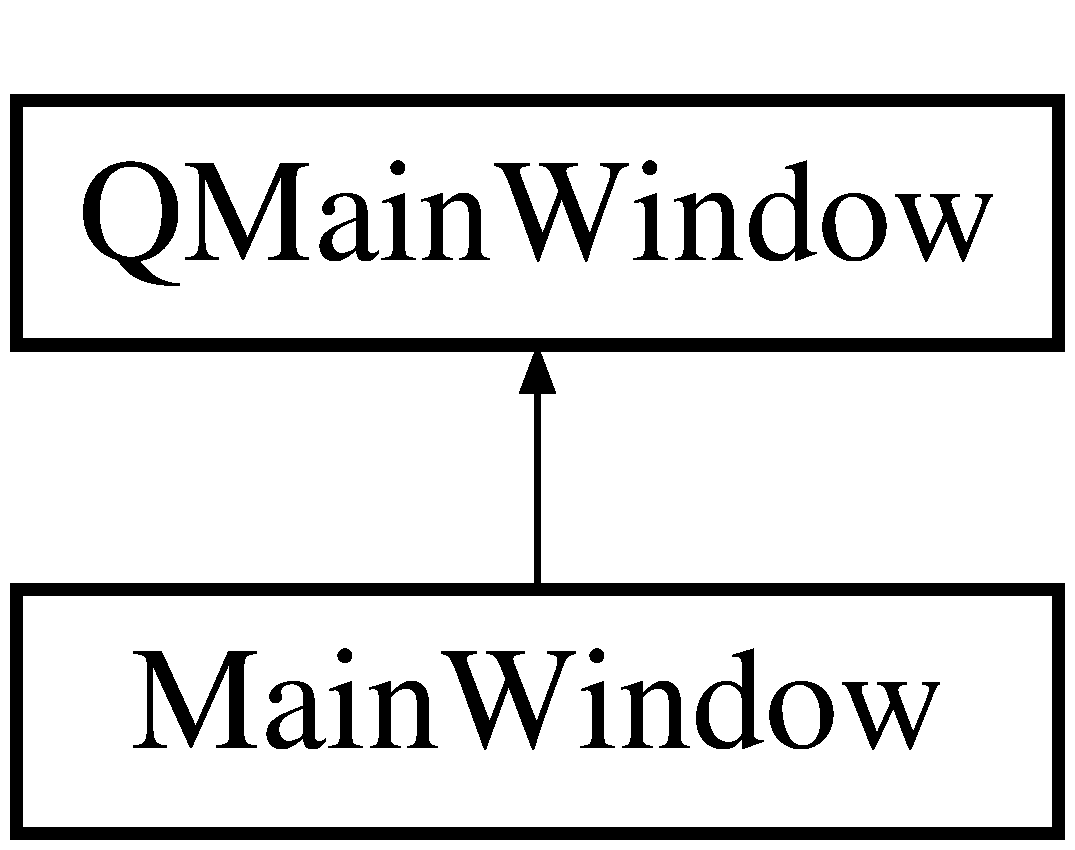
\includegraphics[height=2.000000cm]{class_main_window}
\end{center}
\end{figure}
\subsection*{Public Slots}
\begin{DoxyCompactItemize}
\item 
void \textbf{ tcp\+Connect} (void)
\begin{DoxyCompactList}\small\item\em \doxyref{Main\+Window\+::tcp\+Connect}{p.}{class_main_window_a26b6030035e196b64333906db8302cdd} -\/ Conecta com o servidor. \end{DoxyCompactList}\item 
void \textbf{ tcp\+Disconnect} (void)
\begin{DoxyCompactList}\small\item\em \doxyref{Main\+Window\+::tcp\+Disconnect}{p.}{class_main_window_a3389bbbe4222f115a7609037a1a63bd5} -\/ Disconecta do servidor. \end{DoxyCompactList}\item 
void \textbf{ get\+Data} (void)
\begin{DoxyCompactList}\small\item\em \doxyref{Main\+Window\+::get\+Data}{p.}{class_main_window_ac6d3a5fa8ef8ede69436b9e9a6ee80c1} -\/ Inicia a a captura de dados. \end{DoxyCompactList}\item 
void \textbf{ stop\+Data} (void)
\begin{DoxyCompactList}\small\item\em \doxyref{Main\+Window\+::stop\+Data}{p.}{class_main_window_a2e3dceeb08f18cc1d07e42b79fe7a0c1} -\/ Mata o temporizador e encerra o \doxyref{get\+Data()}{p.}{class_main_window_ac6d3a5fa8ef8ede69436b9e9a6ee80c1};. \end{DoxyCompactList}\item 
void \textbf{ update\+Ip} (void)
\begin{DoxyCompactList}\small\item\em Atualiza lista de clientes produtores conectados. \end{DoxyCompactList}\item 
void \textbf{ timer\+Event} (Q\+Timer\+Event $\ast$e)
\begin{DoxyCompactList}\small\item\em Time event. \end{DoxyCompactList}\end{DoxyCompactItemize}
\subsection*{Public Member Functions}
\begin{DoxyCompactItemize}
\item 
\textbf{ Main\+Window} (Q\+Widget $\ast$parent=0)
\item 
\textbf{ $\sim$\+Main\+Window} ()
\end{DoxyCompactItemize}


\subsection{Constructor \& Destructor Documentation}
\mbox{\label{class_main_window_a8b244be8b7b7db1b08de2a2acb9409db}} 
\index{Main\+Window@{Main\+Window}!Main\+Window@{Main\+Window}}
\index{Main\+Window@{Main\+Window}!Main\+Window@{Main\+Window}}
\subsubsection{Main\+Window()}
{\footnotesize\ttfamily Main\+Window\+::\+Main\+Window (\begin{DoxyParamCaption}\item[{Q\+Widget $\ast$}]{parent = {\ttfamily 0} }\end{DoxyParamCaption})\hspace{0.3cm}{\ttfamily [explicit]}}

\mbox{\label{class_main_window_ae98d00a93bc118200eeef9f9bba1dba7}} 
\index{Main\+Window@{Main\+Window}!````~Main\+Window@{$\sim$\+Main\+Window}}
\index{````~Main\+Window@{$\sim$\+Main\+Window}!Main\+Window@{Main\+Window}}
\subsubsection{$\sim$\+Main\+Window()}
{\footnotesize\ttfamily Main\+Window\+::$\sim$\+Main\+Window (\begin{DoxyParamCaption}{ }\end{DoxyParamCaption})}



\subsection{Member Function Documentation}
\mbox{\label{class_main_window_ac6d3a5fa8ef8ede69436b9e9a6ee80c1}} 
\index{Main\+Window@{Main\+Window}!get\+Data@{get\+Data}}
\index{get\+Data@{get\+Data}!Main\+Window@{Main\+Window}}
\subsubsection{get\+Data}
{\footnotesize\ttfamily void Main\+Window\+::get\+Data (\begin{DoxyParamCaption}\item[{void}]{ }\end{DoxyParamCaption})\hspace{0.3cm}{\ttfamily [slot]}}



\doxyref{Main\+Window\+::get\+Data}{p.}{class_main_window_ac6d3a5fa8ef8ede69436b9e9a6ee80c1} -\/ Inicia a a captura de dados. 

Pega os dados no intervalo de 30 em 30 amostras com um tempo determinado pelo usuário \mbox{\label{class_main_window_a2e3dceeb08f18cc1d07e42b79fe7a0c1}} 
\index{Main\+Window@{Main\+Window}!stop\+Data@{stop\+Data}}
\index{stop\+Data@{stop\+Data}!Main\+Window@{Main\+Window}}
\subsubsection{stop\+Data}
{\footnotesize\ttfamily void Main\+Window\+::stop\+Data (\begin{DoxyParamCaption}\item[{void}]{ }\end{DoxyParamCaption})\hspace{0.3cm}{\ttfamily [slot]}}



\doxyref{Main\+Window\+::stop\+Data}{p.}{class_main_window_a2e3dceeb08f18cc1d07e42b79fe7a0c1} -\/ Mata o temporizador e encerra o \doxyref{get\+Data()}{p.}{class_main_window_ac6d3a5fa8ef8ede69436b9e9a6ee80c1};. 

\mbox{\label{class_main_window_a26b6030035e196b64333906db8302cdd}} 
\index{Main\+Window@{Main\+Window}!tcp\+Connect@{tcp\+Connect}}
\index{tcp\+Connect@{tcp\+Connect}!Main\+Window@{Main\+Window}}
\subsubsection{tcp\+Connect}
{\footnotesize\ttfamily void Main\+Window\+::tcp\+Connect (\begin{DoxyParamCaption}\item[{void}]{ }\end{DoxyParamCaption})\hspace{0.3cm}{\ttfamily [slot]}}



\doxyref{Main\+Window\+::tcp\+Connect}{p.}{class_main_window_a26b6030035e196b64333906db8302cdd} -\/ Conecta com o servidor. 

\mbox{\label{class_main_window_a3389bbbe4222f115a7609037a1a63bd5}} 
\index{Main\+Window@{Main\+Window}!tcp\+Disconnect@{tcp\+Disconnect}}
\index{tcp\+Disconnect@{tcp\+Disconnect}!Main\+Window@{Main\+Window}}
\subsubsection{tcp\+Disconnect}
{\footnotesize\ttfamily void Main\+Window\+::tcp\+Disconnect (\begin{DoxyParamCaption}\item[{void}]{ }\end{DoxyParamCaption})\hspace{0.3cm}{\ttfamily [slot]}}



\doxyref{Main\+Window\+::tcp\+Disconnect}{p.}{class_main_window_a3389bbbe4222f115a7609037a1a63bd5} -\/ Disconecta do servidor. 

\mbox{\label{class_main_window_a9d08a694a5f9c532225754381b8011ea}} 
\index{Main\+Window@{Main\+Window}!timer\+Event@{timer\+Event}}
\index{timer\+Event@{timer\+Event}!Main\+Window@{Main\+Window}}
\subsubsection{timer\+Event}
{\footnotesize\ttfamily void Main\+Window\+::timer\+Event (\begin{DoxyParamCaption}\item[{Q\+Timer\+Event $\ast$}]{e }\end{DoxyParamCaption})\hspace{0.3cm}{\ttfamily [slot]}}



Time event. 

\doxyref{Main\+Window\+::timer\+Event}{p.}{class_main_window_a9d08a694a5f9c532225754381b8011ea} -\/ Configura o temporizador.

função que faz o \doxyref{get\+Data(void)}{p.}{class_main_window_ac6d3a5fa8ef8ede69436b9e9a6ee80c1} ser chamado no tempo determinado pelo usuário


\begin{DoxyItemize}
\item Configura o \doxyref{get\+Data()}{p.}{class_main_window_ac6d3a5fa8ef8ede69436b9e9a6ee80c1} de acordo com o intervalo fornecido pelo usuario 
\end{DoxyItemize}\mbox{\label{class_main_window_a6d5ab019a97676b4edfe7d4b6a541455}} 
\index{Main\+Window@{Main\+Window}!update\+Ip@{update\+Ip}}
\index{update\+Ip@{update\+Ip}!Main\+Window@{Main\+Window}}
\subsubsection{update\+Ip}
{\footnotesize\ttfamily void Main\+Window\+::update\+Ip (\begin{DoxyParamCaption}\item[{void}]{ }\end{DoxyParamCaption})\hspace{0.3cm}{\ttfamily [slot]}}



Atualiza lista de clientes produtores conectados. 

\doxyref{Main\+Window\+::update\+Ip}{p.}{class_main_window_a6d5ab019a97676b4edfe7d4b6a541455} -\/ Atualiza a lista de produtores conectados. 

The documentation for this class was generated from the following files\+:\begin{DoxyCompactItemize}
\item 
\textbf{ mainwindow.\+h}\item 
\textbf{ mainwindow.\+cpp}\end{DoxyCompactItemize}

%--- End generated contents ---

% Index
\backmatter
\newpage
\phantomsection
\clearemptydoublepage
\addcontentsline{toc}{chapter}{Index}
\printindex

\end{document}
